\documentclass[11pt,a4paper]{article}

\usepackage[margin=2.5cm]{geometry} % Margin
\usepackage{graphicx}
\usepackage[ansinew]{inputenc}

\title{A Short Tutorial on DeerAnalysis2010}
\author{G. Jeschke \\ \emph{ETH Z\"urich, Lab. Phys. Chem., Wolfgang-Pauli-Strasse 10, CH-8093 Z\"urich, Switzerland} \\ gjeschke@ethz.ch}

\begin{document}

\maketitle

\section{Preface}

This tutorial describes analysis of distance measurements by pulsed ELDOR \cite{milov1981,milovrev}, specifically by the four-pulse DEER experiment \cite{pannier2000,jeschke2002,jeschkerev}, with the program DeerAnalysis2010. The program is based on algorithms discussed previously \cite{jeschke2001,jeschke2004,chiang2005} and on some new algorithms. A discussion of the main algorithms, except for validation, is given in \cite{jeschke2006}. The program requires Matlab and can be downloaded at http://www.epr.ethz.ch/software/index. If you have a Matlab version older than Matlab 2008, you need to work with DeerAnalysis2006, which has the same user interface and functionality, except for validation. This program can be downloaded from the same homepage. For experimental aspects of optimizing the DEER experiment, i.e. for ways to obtain the best possible input data for DeerAnalysis, you may consult \cite{jeschke2007}.

\section{Worked example: A single well-defined distance}

\subsection{Basic Tikhonov processing}

Example data for worked examples and set tasks are found in the {\ttfamily tutorial} subdirectory of {\ttfamily DeerAnalysis}

\begin{itemize}
	\item Load file {\ttfamily deer\_3\_6nm\_50K} DeerAnalysis automatically corrects the phase and tries to determine zero time.
	\item In the present example, zero time should be 96 ns, but the program finds 111 ns.\footnote{We know that from other measurements with the same spectrometer, probehead, and pulse sequence timings. The zero time for such a given configuration can be determined most precisely with a model compound with a short distance measured with high signal-to-noise ratio.} Correct the value to 96 ns, using the green {\ttfamily -} button in the {\ttfamily \bf Original data} panel.
	\item As data were measured until almost complete decay, the {\ttfamily \bf Form factor} is rather noisy.\footnote{With more experience, we would not have measured like that. The sample should have been diluted, see \cite{jeschke2007}} Cut the data by repeatedly clicking on the brown {\ttfamily !} button in the {\ttfamily \bf Original data} panel.
	\item Optimize the range for the background fit by clicking on the blue {\ttfamily !} button in the {\ttfamily \bf Original data} panel. This will take some time. You can follow progress in the {\ttfamily \bf Status} line (left bottom).
	\item In the {\ttfamily \bf Distance analysis} panel, select the {\ttfamily Tikhonov} radio button. Click on the {\ttfamily Fit} button right from the radiobutton. Fitting will also take some time, as this data set is very long.
\end{itemize}

The plot panels should now look as shown in Figure \ref{fig:1}.

\begin{figure}[ht]
 \vspace{10mm}
 	\begin{center}
		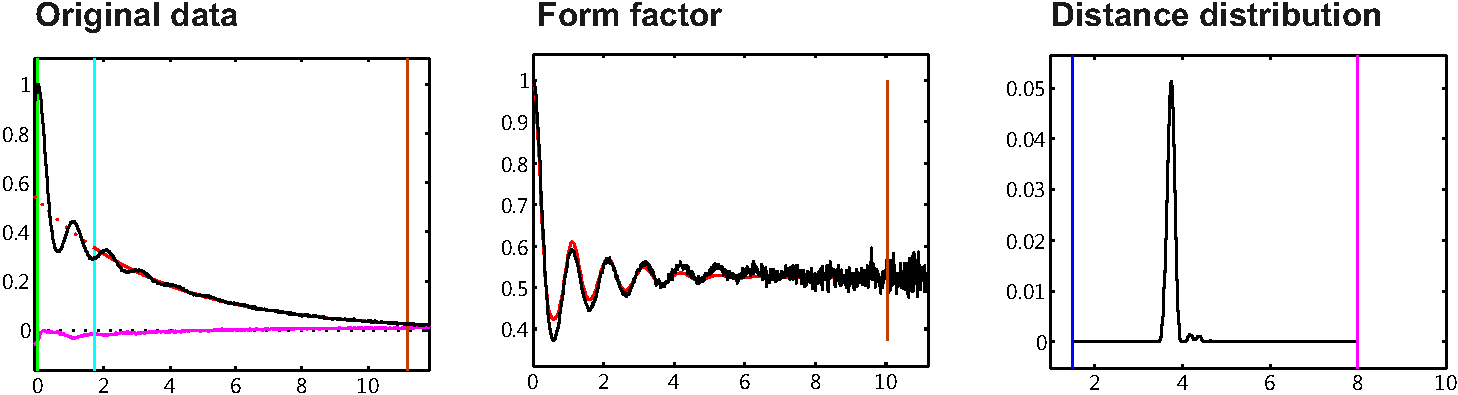
\includegraphics[width=0.95\textwidth]{figure1.pdf}
	\end{center}
	\caption{Plots in DeerAnalysis2010 after basic Tikhonov processing of file {\ttfamily deer\_3\_6nm\_50K}.}
	\label{fig:1}
\end{figure}

They provide the following information:

\subsubsection*{Original data}
\begin{itemize}
	\item \emph{Black trace}: real part of the primary experimental data after phase correction.
	\item \emph{Magenta trace}: imaginary part of the primary experimental data after phase correction.\footnote{Ideally, this is a flat line at zero. Any deviation indicates some problem with the spectrometer or imperfect phase correction.}
	\item \emph{Green cursor}: current setting of zero time.
	\item \emph{Light blue cursor}: start of the range for background fitting.
  \item \emph{Brown cursor}: cutoff of the data at the end and end of the range for background fitting.
  \item \emph{Red trace}: fitted background function, solid line within the fit range, dotted line outside the fit range (extrapolation). 
\end{itemize}

\subsubsection*{Form factor}
\begin{itemize}
	\item \emph{Black trace}: form factor (dipolar evolution function after background correction, i.e. divided by background function and renormalized).
	\item \emph{Red trace}: fit of the dipolar evolution function corresponding to the displayed distance distribution.
	\item \emph{Brown cursor}: suggested cutoff time.
\end{itemize}

Note that the suggested cutoff time is different from the cutoff time originally used in Tikhonov regularization. This is because Tikhonov regularization provides a better fit to the data than the original APT (approximate Pake transformation) result. Thus, the noise level can be estimated more precisely and it can be judged more precisely, at which dipolar evolution time experimental noise becomes too large.

\subsubsection*{Distance distribution}
\begin{itemize}
	\item \emph{Black trace}: distance distribution computed by the currently selected technique for data analysis (here Tikhonov regularization).
	\item \emph{Blue cursor}: lower end of the fit range or range for data analysis.
	\item \emph{Magenta cursor}: upper end of the fit range or range for data analysis.
\end{itemize}

The mean distance $\langle r \rangle$ (3.80 nm) and the width of the distance distribution, given as standard deviation $s(r)$ (0.19 nm), are displayed in the panel {\ttfamily \bf Distance analysis}.

\subsection{Inspecting data}

The plots can be changed to allow for closer inspection. For instance, the {\ttfamily \bf Original data} (real part) are somewhat better seen when switching off the imaginary part (click on the {\ttfamily imaginary} checkbox). The other two plots can be adapted more extensively. 

\subsubsection*{Form factor}
\begin{itemize}
	\item \emph{Closer inspection of the initial part}: Click on the $<>$ button in the {\ttfamily Zoom} subpanel. Each click expands the initial part of the evolution function by a factor of $\sqrt{2}$. The $><$ button reduces zoom in the same way. The {\ttfamily !} button resets zoom to 1.0.
	\item \emph{Dipolar spectrum}: Select the {\ttfamily Spectrum} radiobutton. The Fourier transform of the baseline-corrected dipolar evolution function (black trace) and its fit corresponding to the computed distance distribution (red trace) are shown. The {\ttfamily Zoom} button $<>$ expands the range around zero frequency (Figure \ref{fig:2}). The zoom factor can also be input directly in the edit field.
\end{itemize}

\begin{figure}[ht]
 \vspace{10mm}
 	\begin{center}
		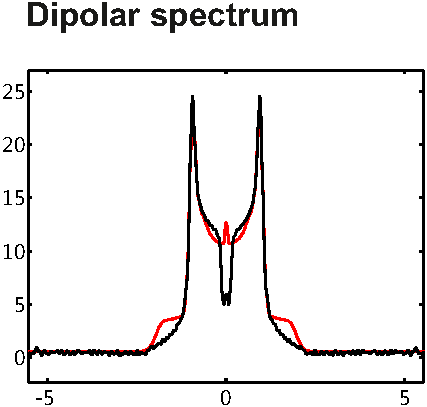
\includegraphics[width=0.30\textwidth]{figure2.pdf}
	\end{center}
	\caption{Dipolar spectrum of data set {\ttfamily deer\_3\_6nm\_50K} at zoom factor 5.7.}
	\label{fig:2}
\end{figure}

You should always take a look at the dipolar spectrum. In the case at hand you see that shoulders of the Pake pattern are missing. This is due to orientation selection. It is also the main reason for deviation of the simulated from the experimental dipolar evolution function in the middle panel of Figure \ref{fig:1}. The problem could have been solved experimentally by averaging DEER measurements taken at different magnetic fields \cite{godt2006}. The hole in the center of the Pake pattern indicates overcorrection of the background.

\subsubsection*{Distance distribution}
\begin{itemize}
	\item \emph{Expand}: To inspect the peak more closely, click on the {\ttfamily Expand} checkbox. Only the range between the cursors is now displayed. Select {\ttfamily 3} nm in the edit field {\ttfamily Start} and {\ttfamily 5} nm in the edit field {\ttfamily End} (Figure \ref{fig:3}). 
\end{itemize}

The main peak is situated between 3.5 and 3.9 nm. It is slightly asymmetric (steeper slope towards long distances).\footnote{for the reason, see \cite{godt2006}} There are some further peaks between 4 and 4.5 nm. To exclude them from analysis, select {\ttfamily 3.5} nm in the edit field {\ttfamily Start} and {\ttfamily 4.0} nm in the edit field {\ttfamily End}. The values in the panel {\ttfamily \bf Distance analysis} change to $\langle r \rangle = 3.75$ nm and $s(r) = 0.08$ nm.

\begin{figure}[ht]
 \vspace{10mm}
 	\begin{center}
		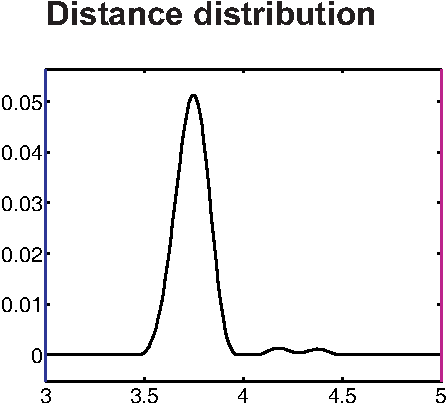
\includegraphics[width=0.30\textwidth]{figure3.pdf}
	\end{center}
	\caption{Range of interest from 3.0 to 5.0 nm in the distance distribution for data set {\ttfamily deer\_3\_6nm\_50K}.}
	\label{fig:3}
\end{figure}

\begin{itemize}
\item \emph{Testing for the relevance of peaks}: Uncheck the checkbox expand. The whole distribution is shown again. Select {\ttfamily 5.0} nm in the edit field {\ttfamily End} and {\ttfamily 4.00} nm in the edit field {\ttfamily Start}. Now click on the green {\ttfamily Suppress button}. Select the {\ttfamily Time domain} radiobutton in the panel {\ttfamily \bf Form factor} and set the zoom to 1.0 ({\ttfamily !} button) (Figure \ref{fig:4}). 
\end{itemize}

\begin{figure}[ht]
 \vspace{10mm}
 	\begin{center}
		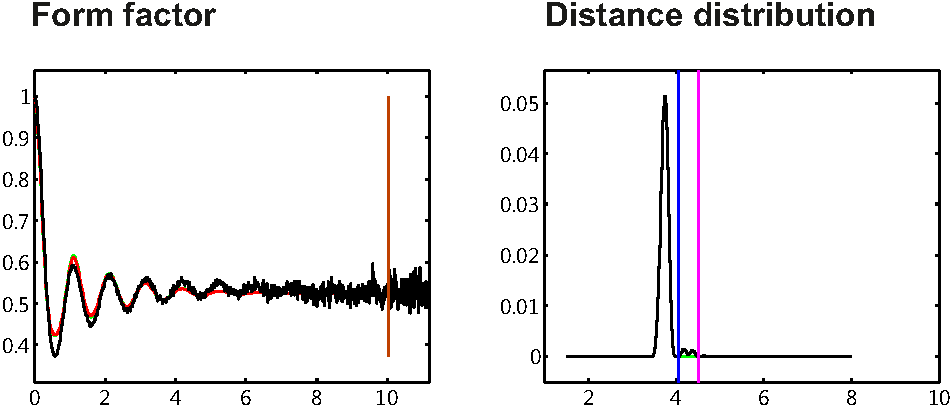
\includegraphics[width=0.62\textwidth]{figure4.pdf}
	\end{center}
	\caption{Test for the relevance of small contributions to the distance distribution. The green traces correspond to supression of the peaks between the blue and magenta cursor.}
	\label{fig:4}
\end{figure}

In the case at hand, supression of the small peaks does not significantly change the quality of the fit of the {\ttfamily \bf Form factor}. The green trace hardly deviates from the red one. These small peaks are thus noise-related. We shall see later how such tests can be performed more thoroughly with the validation tool. 

\subsection{Using the L curve for optimized Tikhonov regularization}

Before attempting a new fit, you need to reset the {\ttfamily \bf Distance distribution} cursors to their default values.\footnote{Otherwise, Tikhonov regularization is restricted to the distance range between cursors. This is an advanced feature, in most cases such restriction will produce nonsensical output.} This can be done by clicking on the blue and magenta {\ttfamily !} buttons in that panel. The values should change to 1.5 and 8.0 nm.

\begin{itemize}
\item \emph{Computing the L curve}: Confirm that the radiobutton {\ttfamily Tikhonov} in the {\ttfamily \bf Distance analysis} panel is selected. Select the checkbox {\ttfamily Compute L curve} and click on the {\ttfamily Fit} button. Tikhonov regularization is performed for regularization parameters $\alpha =$ 0.001, 0.01, 0.1, 1, 10, 100, 1000, 10000, and 100000.\footnote{\emph{Trick:}You can have any set of $\alpha$ values you want. For that you need to edit the file {\ttfamily Lcurve\_abscissa.dat} in the main directory of DeerAnalysis.} The status line shows the currently computed data set. The {\ttfamily \bf Form factor} fit (red line) and {\ttfamily \bf Distance distribution} are updated after computation for each individual regularization parameter. The whole series of computations takes several minutes. Finally, the {\ttfamily L curve} checkbox in the {\ttfamily \bf Distance distribution} panel is automatically selected and the L curve displayed. A red dot marks the point where the program locates the corner of the L curve.\footnote{The program guesses the corner. Sometimes, as in this case, you may be able to locate it more precisely "by eye"} (Figure \ref{fig:5}a) 
\item \emph{Navigating the L curve}: To select a data set corresponding to a different point in the L curve (different regularization parameter), use the black {\ttfamily Reg. par. +} and {\ttfamily -} buttons in the {\ttfamily \bf Distance distribution} panel. The value of the regularization parmeter, the fit in the {\ttfamily \bf Form factor} plot and the {\ttfamily r.m.s.} value, $\langle r \rangle$, and $s(r)$ in the {\ttfamily \bf Distance analysis} panel update.
\end{itemize}

In the case at hand, regularization parameters of 1 or larger correspond to overdamping of the {\ttfamily \bf Form factor}, i.e., to oversmoothing of the distance distribution. A regularization parameter $\alpha = 0.1$ is the optimum choice (Figure \ref{fig:5}c,d). At even smaller regularization parameters, the fit and r.m.s. value improve only insignificantly. The distance distributions corresponding to all computed values of $\alpha$ can be inspected by unchecking the {\ttfamily L curve} checkbox in the {\ttfamily \bf Distance distribution} panel and using the black {\ttfamily Reg. par. +} and {\ttfamily -} buttons for selection.

\begin{figure}[ht]
 \vspace{10mm}
 	\begin{center}
		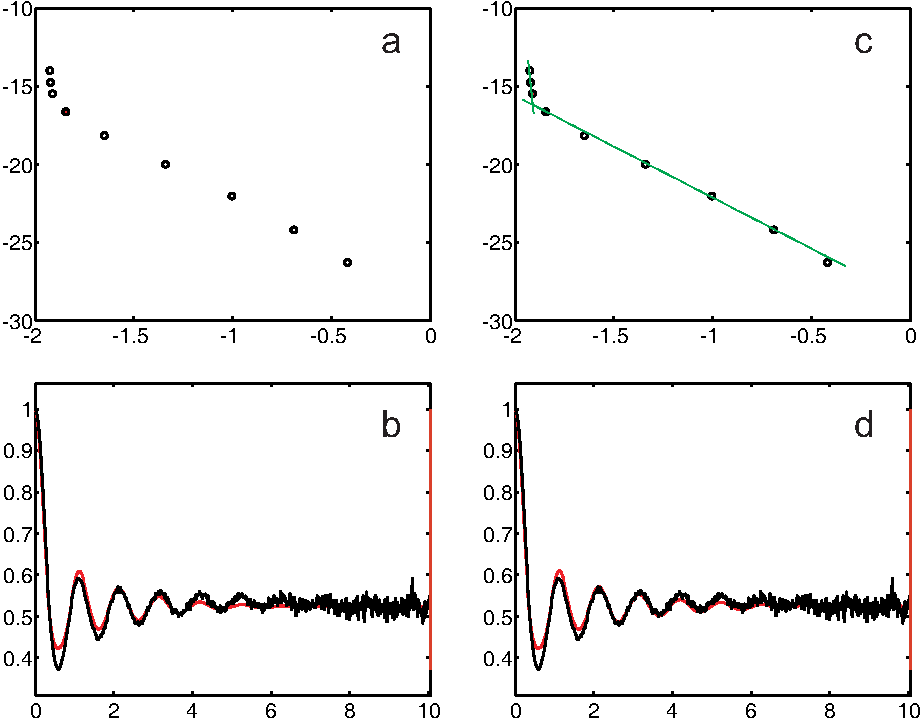
\includegraphics[width=0.62\textwidth]{figure5.pdf}
	\end{center}
	\caption{L curve for the data set {\ttfamily deer\_3\_6nm\_50K}. a) Corner suggested by the program (red dot). b) Fit corresponding to selection by the program. c) Corner selected by visual inspection (red dot). The green dotted lines are guides to the eye, added in a drawing program. d) Fit corresponding to visual selection. }
	\label{fig:5}
\end{figure}

\section{Problem set: Two peaks}

\subsection{Problem}

Perform an analysis of the data set {\ttfamily DEER\_mix\_50K}, using Tikhonov regularization with L curve computation (Figure \ref{fig:6}). In contrast to the example above, do not change the automatically determined zero time. Give
\begin{enumerate}
	\item the optimum regularization parameter
	\item distance and width (standard deviation) for the first peak
	\item distance and width (standard deviation) for the second peak
\end{enumerate}

\begin{figure}[ht]
 \vspace{10mm}
 	\begin{center}
		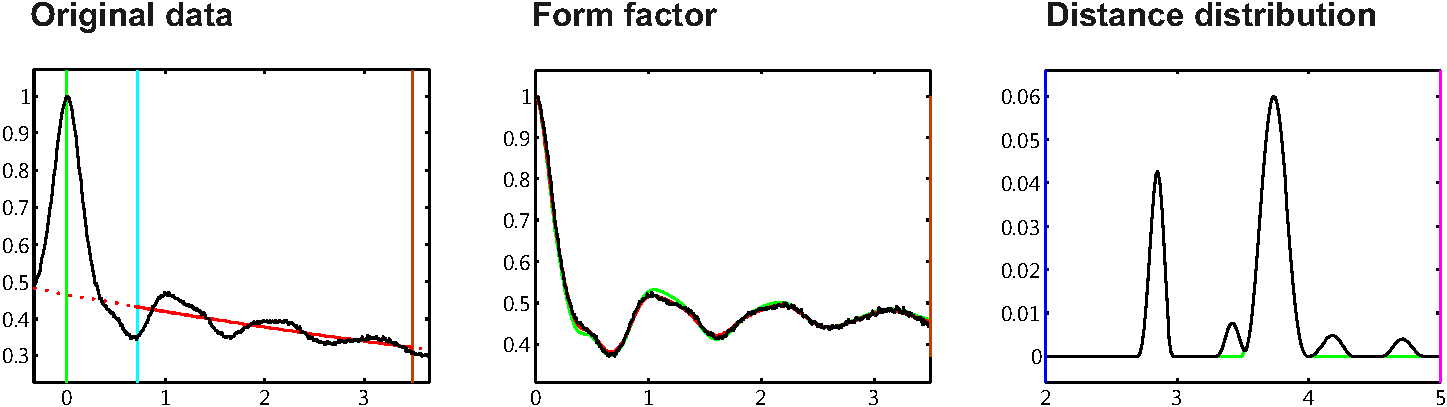
\includegraphics[width=0.95\textwidth]{figure6.pdf}
	\end{center}
	\caption{Result of Tikhonov regularization ($\alpha = 0.1$) for the data set {\ttfamily DEER\_mix\_50K}. }
	\label{fig:6}
\end{figure}
    
\subsection{Answer}

1) $\alpha = 0.1$. 2) $\langle r \rangle = 2.84$ nm, $s(r) = 0.05$ nm. 3) $\langle r \rangle = 3.72$ nm, $s(r) = 0.10$ nm. One can argue about the correct interval for the second peak and about suppression of the small peaks. The small peaks are not related to noise, but probably to errors in background correction and to orientation selection artefacts. 
    
\section{Worked example: Gaussian fitting}

\subsection{Background correction as pre-processing}

Whenever a reasonable correction of the intermolecular background can be made, it should be made before fitting the dipolar evolution rather than fitting the intramolecular and intermolecular distance distributions simultaneously. This is demonstrated in the following.

\begin{itemize}
	\item Load (or reload) data set {\ttfamily DEER\_mix\_50K}. This resets all controls of {\ttfamily DeerAnalysis2010} to their default values.
	\item In panel {\ttfamily \bf Distance analysis} select the radiobutton {\ttfamily Model fit} and from the popup menu to the right the model {\ttfamily Two Gaussians}. The {\ttfamily \bf Distance distribution} plot displays the result of an APT (black dashed line) and the modelled distribution (red dashed line), using the starting values for the mean distance of the first peak $\langle r1 \rangle$, the width (standard deviation) of the first peak $s(r1)$, the relative contribution (integral) $p1$ of the first peak, the mean distance of the second peak $\langle r2 \rangle$, and the width (standard deviation) of the second peak $s(r2)$. The fit of the {\ttfamily \bf Form factor} data is shown as a red dotted curve.
	\item Improve the starting values by direct input into the edit fields. Good starting values decrease the probability to end up in a local minimum of the error hypersurface. Use the black APT curve in the {\ttfamily \bf Distance distribution} plot as a guide for changing the parameters. Good values are $\langle r1 \rangle = 2.8$ nm, $s(r1) = 0.2$ nm, $p1 = 0.3$, $\langle r2 \rangle = 3.75$ nm, $s(r2) = 0.2$ nm. When finished, click on the {\ttfamily Fit} button in the {\ttfamily Model fit} subpanel. The status line shows how the r.m.s. value changes during fitting.
	 \item When the fit is completed, the {\ttfamily \bf Distance distribution} plot updates to a black solid line, corresponding to the model of two Gaussian peak. The {\ttfamily \bf Form factor} data corresponding to this distribution is now shown as a red solid line (Figure \ref{fig:7}).
\end{itemize}

\begin{figure}[ht]
 \vspace{10mm}
 	\begin{center}
		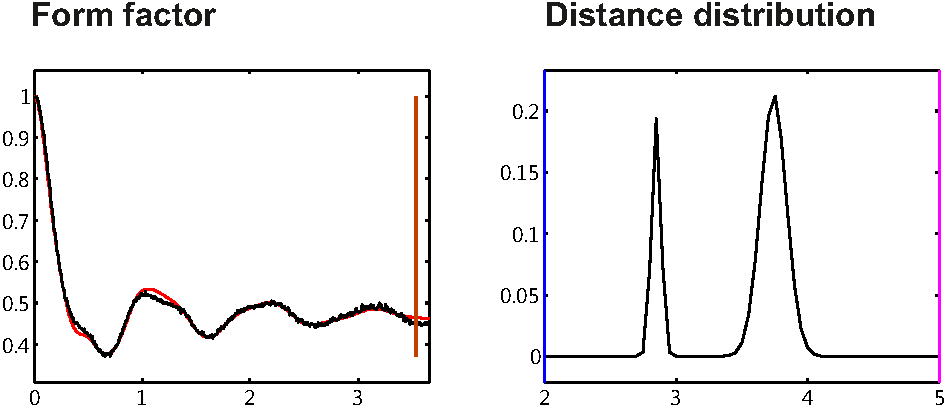
\includegraphics[width=0.62\textwidth]{figure7.pdf}
	\end{center}
	\caption{Result of model fitting with two Gaussian peaks for the problem data set {\ttfamily DEER\_mix\_50K}. }
	\label{fig:7}
\end{figure}

You should find the values $\langle r1 \rangle = 2.85$ nm, $s(r1) = 0.05$ nm, $p1 = 0.26$, $\langle r2 \rangle = 3.74$ nm, $s(r2) = 0.13$ nm. Slight differences may arise from background correction and cutoff setting.

\subsection{Simultaneous fit of background and distance distribution}

\begin{itemize}
	\item Change the {\ttfamily \bf Background model} to {\ttfamily No correction} and from the popup menu in the {\ttfamily Model fit} subpanel select {\ttfamily Two\_Gaussians\_hom}. Adjust the starting parameters as above. Finally adjust the concentration parameter $c$, so that the dotted red fit in the {\ttfamily \bf Form factor} panel is reasonable. You should find a value of $c \approx 0.4$.
	\item Click on the {\ttfamily Fit} button. With this good set of starting parameters the program finds a reasonable solution (Figure \ref{fig:8}: $\langle r1 \rangle = 2.84$ nm, $s(r1) = 0.06$ nm, $p1 = 0.27$, $\langle r2 \rangle = 3.73$ nm, $s(r2) = 0.17$ nm, $c = 0.36$). Note that the displayed distance distribution now contains a background contribution. In the case at hand this contribution shows that intermolecular interactions are relevant already at the distance of the second peak. The sample should be diluted to improve the results. 
\end{itemize}

\begin{figure}[ht]
 \vspace{10mm}
 	\begin{center}
		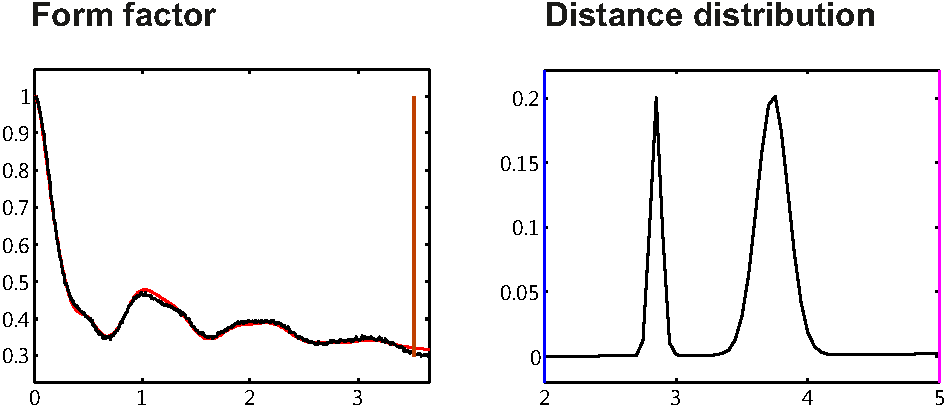
\includegraphics[width=0.62\textwidth]{figure8.pdf}
	\end{center}
	\caption{Result of model fitting with two Gaussian peaks plus homogeneous background for the problem data set {\ttfamily DEER\_mix\_50K}. }
	\label{fig:8}
\end{figure}

Simultaneous background fitting is, however, less stable.

\begin{itemize}
	\item Again fit the model {\ttfamily Two\_Gaussians\_hom} using the {\ttfamily No correction as \bf Background model}, but now with the slightly worse starting parameters $\langle r1 \rangle = 2.7$ nm, $s(r1) = 0.3$ nm, $p1 = 0.5$, $\langle r2 \rangle = 4.0$ nm, $s(r2) = 0.3$ nm, $c=0.4$. The program finds a local minimum with a very broad first peak.  
	\item Repeat the fit {\ttfamily Two\_Gaussians} using the {\ttfamily Homogeneous \bf Background model} with three dimensions, with the same starting parameters $\langle r1 \rangle = 2.7$ nm, $s(r1) = 0.3$ nm, $p1 = 0.5$, $\langle r2 \rangle = 4.0$ nm, $s(r2) = 0.3$ nm. The program finds the same fit as with the better starting parameters.  
\end{itemize}

The message is that model fitting becomes the more delicate the more fit parameters you have. Whenever you have enough information to separate a large fit problem (distance distribution and background) into two smaller ones (first background, then distance distribution), do so. For DEER data, if you do not feel confident with fitting the background separately, it is rather unlikely that simultaneous fitting of background and distance distribution will give a stable and reliable result. You then need to improve experimental data or, if this is impossible, interpret data very cautiously.

\subsection{Problem: Fitting a single Gaussian peak}

\subsubsection*{Problem}

Load the spectrum {\ttfamily deer\_long\_50K}. Adjust zero time to 96 ns and optimize the fit range for background correction. Set the magenta {\ttfamily End} cursor to an appropriate distance $r_\mathrm{end}$ and fit the distance distribution after background correction by a single Gaussian peak (model {\ttfamily Gaussian}). Give $r_\mathrm{end}$ and the fit parameters.

\subsubsection*{Answer}
$r_\mathrm{end} = 10$ nm, $\langle r \rangle = 7.52$ nm, $s(r) = 0.31$ nm.

\section{Worked example: Very broad distance distribution}

\subsection{Assuming ideal pulses}
Data set {\ttfamily deer\_broad\_50K\_4us} was measured on a sample of surface-labelled gold nanoparticles. Assuming spherical nanoparticles with a well-defined diameter $d$ and a constant distance of the nitroxide labels from the surface, the distribution of distances $P(r)$ between labels on the surface of the same particle would be shaped as a sawtooth (triangular), increasing linearly as $P(r)= k r$ for $0 \leq r \leq d$, and being identical zero for $r > d$ (see Figure \ref{fig:9}d).

\begin{figure}[ht]
 \vspace{10mm}
 	\begin{center}
		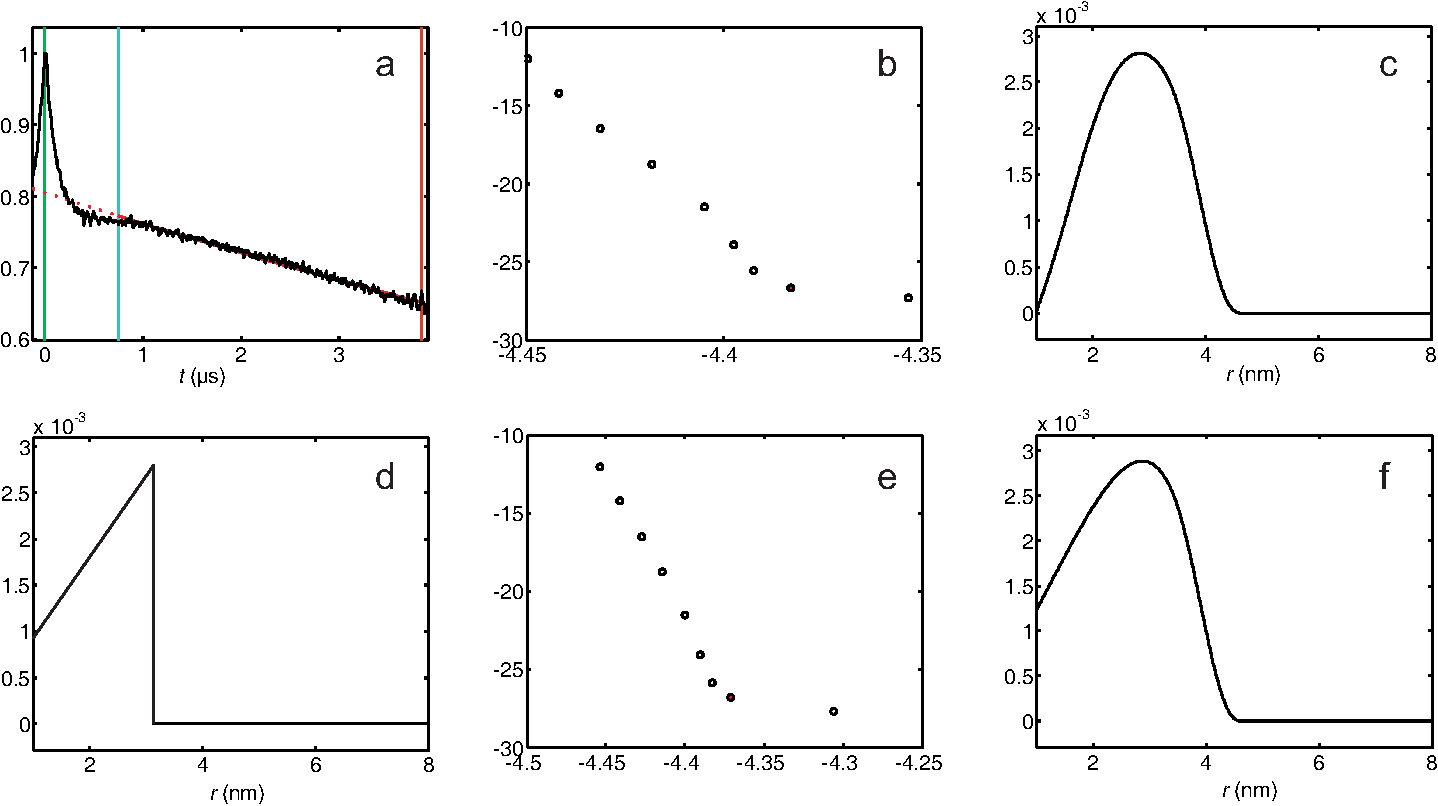
\includegraphics[width=0.95\textwidth]{figure9.pdf}
	\end{center}
	\caption{Analysis of data set {\ttfamily deer\_broad\_50K\_4us} corresponding to a distribution of spin labels on the surface of a gold nanoparticle. (a) Original data with background fit. (b) L curve of Tikhonov regularization assuming ideal pulses. The red dot marks the optimum regularization parameter $\alpha = 10000$. (c) Distance distribution at $\alpha = 10000$ assuming ideal pulses. (d) Schematic distance distribution, assuming monodisperse, ideally spherical gold nanoparticles and a uniform distance of the labels from the surface. (e) L curve of Tikhonov regularization with correction for limited excitation bandwidth of the pulses. The red dot marks the optimum regularization parameter $\alpha = 10000$. (f) Distance distribution at $\alpha = 10000$ with excitation bandwidth correction.}
	\label{fig:9}
\end{figure}

\begin{itemize}
	\item Load data set {\ttfamily deer\_broad\_50K\_4us}. Set the magenta {\ttfamily Start} cursor in the {\ttfamily \bf Distance distribution} to 1.0 nm. Optimize the fit range for the background (Figure \ref{fig:9}a).
	\item Compute the L curve for Tikhonov regularization. The corner of the L curve is at $\alpha = 10000$. Select this regularization parameter. (Figure \ref{fig:9}b).
	\item Switch to the distance distribution (Figure \ref{fig:9}c). It is approximately zero at $r=1.0$ nm. Why?  
\end{itemize}

\subsection{Correcting for limited excitation bandwidth}
The microwave pulses in the DEER experiment have limited excitation bandwidth. If the dipole-dipole coupling between the two spins is of the same order as or even larger than the excitation bandwidth, the dipolar modulation is suppressed. This can be accounted for by assuming an excitation profile with Gaussian shape and with a width that depends on the width of the pulses in the DEER sequence. For observer pulses of 32 ns length and a pump pulse of 12 ns length, the excitation bandwidth is 16 MHz, the default value in DeerAnalysis2010.      

\begin{itemize}
	\item Select the {\ttfamily Exci. bandwidth} checkbox in the {\ttfamily \bf Form factor} panel and repeat computation of the L curve for Tikhonov regularization. \emph{Warning:} This may take \emph{very} long. The shape of the L curve improves (compare Figure \ref{fig:9}b and e).
	\item Switch to the distance distribution (Figure \ref{fig:9}f). The remaining deviations from a triangular shape can be traced back to the size dispersion of the nanoparticles, to the conformational distribution of the spin labels on the surface, and apparently to some overcompensation of the lost modulation.  
\end{itemize}

Even with excitation bandwidth correction, DEER has a limitation towards short distances. Therefore, DeerAnalysis2010 does not allow for extending the distance range for analysis below 1.0 nm. Contributions in the range between 1.0 and 1.5 nm should be interpreted with utmost caution.

In the case at hand, the general shape of the distance distribution is approximately known, it is a sawtooth function convoluted with a Gaussian (distribution of nanoparticle size). If this knowledge is used (fit model {\ttfamily Sphere\_Surface} \emph{without} excitation bandwidth correction), suppression of short distances is less of a problem. In addition, the parameters have a clear physical meaning. If you believe that you have a good model for a distance distribution, it is good practice to first check whether results from Tikhonov regularization are consistent with that model and then use a fit of the model to time-domain data to extract parameters. Do not fit the model to the distance distribution obtained after Tikhonov regularization.\footnote{See the manual of {\ttfamily DeerAnalysis} on how to specify your own model with up to 8 parameters in terms of a distance distribution}

\section{Worked example: Dual display}

In many applications it is of interest whether or not the distance distribution between two spin labels changes. Since conversion of dipolar evolution functions to distance distributions is an ill-posed problem, such comparisons should always be made on the original time-domain data. Changes in the distance distribution should only be discussed after it is established that original data are significantly different. Otherwise, they might be noise-related. For comparing original data sets, data sets after background correction, and distance distributions of two samples, DeerAnalysis2010 features a dual display.

\subsection{A case with no significant difference}

\begin{figure}[ht]
 \vspace{10mm}
 	\begin{center}
		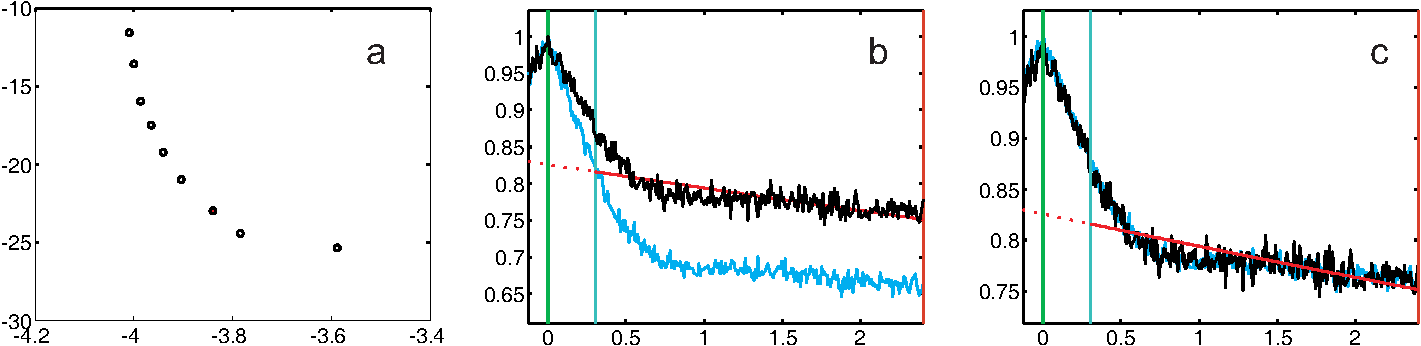
\includegraphics[width=0.95\textwidth]{figure10.pdf}
	\end{center}
	\caption{Dual display processing of data sets {\ttfamily LHCIIb\_1} and {\ttfamily LHCIIb\_2}. (a) L curve for data set {\ttfamily LHCIIb\_1}. The red dot shows the estimated optimum regularization parameter. (b) Original data sets {\ttfamily LHCIIb\_2} (black) and {\ttfamily LHCIIb\_1} (blue). The background fit corresponds to the active data set (black). (c) Original data sets after modulation depth scaling.}
	\label{fig:10}
\end{figure}

\begin{itemize}
	\item Load data set {\ttfamily LHCIIb\_1}, which is a measurement on mutant S106R1/S160R1 of light harvesting complex IIb with a particular pigment mixture. Set zero time to 128 ns, optimize the range for background fitting, and perform L curve computation for Tikhonov regularization. The corner of the L curve is difficult to determine. By looking at the fits of the {\ttfamily \bf Form factor} data for different values of the regularization parameter $\alpha$, one finds that $\alpha = 1000$ is a reasonable choice (Figure \ref{fig:10}a).
	\item Load data set {\ttfamily LHCIIb\_2}, which is a measurement on the same mutant but with a different pigment mixture. In the {\ttfamily \bf Data sets} panel, the newly loaded data is now set {\ttfamily A:} (black) and the previously loaded data is set {\ttfamily B:} (blue). Again set zero time to 128 ns, optimize the range for background fitting, and perform L curve computation for Tikhonov regularization. Select $\alpha = 1000$ (this is a case where the L curve is misleading), and uncheck the {\ttfamily L curve} checkbox in the {\ttfamily Distance distribution} panel. 
	\item Now select the {\ttfamily Dual display} checkbox in the {\ttfamily \bf Original data} panel. Data set {\ttfamily B:} is displayed as a blue trace in all three plots (Figure \ref{fig:10}b). The black and blue traces do not agree. This could be due to either of the following reasons: (a) different degree of spin labeling and thus different modulation depth or (b) a change in the distance distribution.
	\item To suppress effects of different modulation depth, select the {\ttfamily mod. depth scaling} checkbox in the {\ttfamily Original data} panel. There is no longer a significant difference between the original data (Figure \ref{fig:10}c). Any difference that can be seen between the distance distributions is due to noise.    
\end{itemize}

\subsection{A case with significant difference}

\begin{figure}[ht]
 \vspace{10mm}
 	\begin{center}
		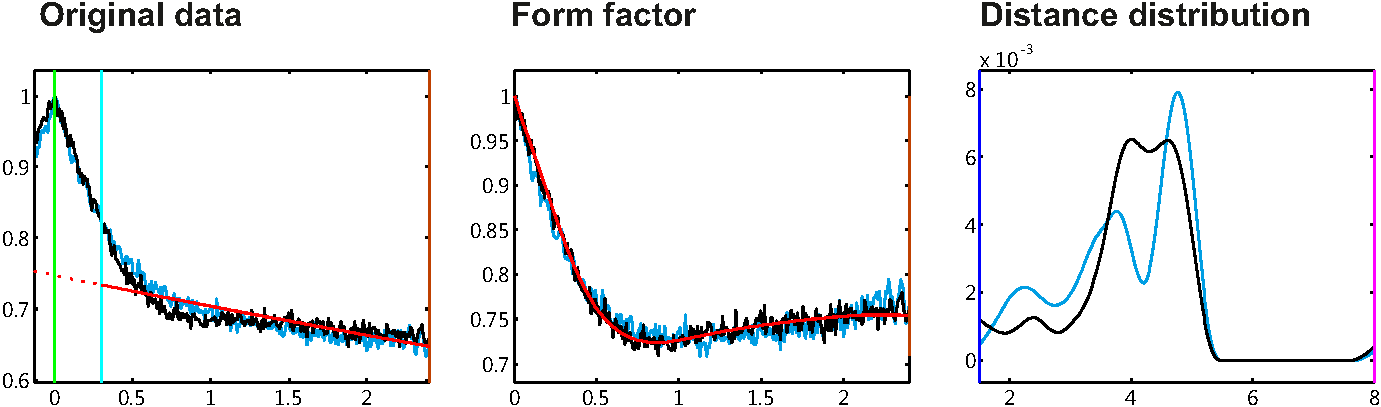
\includegraphics[width=0.95\textwidth]{figure11.pdf}
	\end{center}
	\caption{Dual display processing of data sets {\ttfamily LHCIIb\_1} and {\ttfamily LHCIIb\_3} with modulation depth scaling.}
	\label{fig:11}
\end{figure}

\begin{itemize}
	\item Now load data set {\ttfamily LHCIIb\_3}, corresponding to yet another pigment mixture. DeerAnalysis2010 reverts to the normal display mode. In the {\ttfamily \bf Data sets} panel, the data set {\ttfamily A:} (black) is now {\ttfamily LHCIIb\_3} and data set {\ttfamily B:} (blue) becomes {\ttfamily LHCIIb\_2}. Data set {\ttfamily LHCIIb\_1} is discarded.
	\item Set zero time to 128 ns, optimize the range for background fitting, and perform L curve computation for Tikhonov regularization. Here, a regularization parameter of $\alpha = 100$ or even $\alpha = 10$ might be appropriate, but for the sake of comparison also select $\alpha = 1000$. Uncheck the {\ttfamily L curve} checkbox in the {\ttfamily \bf Distance distribution} panel.
	\item Select the {\ttfamily Dual display} and {\ttfamily mod. depth scaling} checkboxes in the {\ttfamily \bf Original data} panel. The difference is subtle, but it is there.  
	\item Load data set {\ttfamily LHCIIb\_1} and repeat the procedure. The difference can be seen much better with this data set, as it has better signal-to-noise ratio than data set {\ttfamily LHCIIb\_2} (Figure \ref{fig:11}).\footnote{\emph{Trick:}The difference can be seen even better when you detach the plots with the {\ttfamily Copy} button in the {\ttfamily \bf Data sets} panel and maximize the figures}  
\end{itemize}

\section{Spin counting via the modulation depth}

The pump pulse in a DEER experiment excites only a fraction of the spins B coupled to the observer spin A. Therefore, only a fraction of the echo is modulated, the modulation depth $\lambda$ is smaller than unity. If several B spins are coupled to the same A spin there is a higher probability that the pump pulse excites at least one of these spins and the modulation depth is thus larger. If all the other parameters that influence modulation depth (pulse lengths, flip angle of the pump pulse, spectral line shape of the nitroxide) are kept constant, the number of coupled spins in a nanoobject can thus be counted \cite{milov1984,hilger2005,bode2007}. Unless the nanoobjects are highly diluted, a proper background correction is needed before the modulation depth is determined \cite{jeschke2004}. DeerAnalysis2010 incorporates the mathematics that are needed to convert background-corrected modulation depths to the number of coupled spins. For a detailed analysis of this problem and possible pitfalls see \cite{bode2007}.

\begin{figure}[ht]
 \vspace{10mm}
 	\begin{center}
		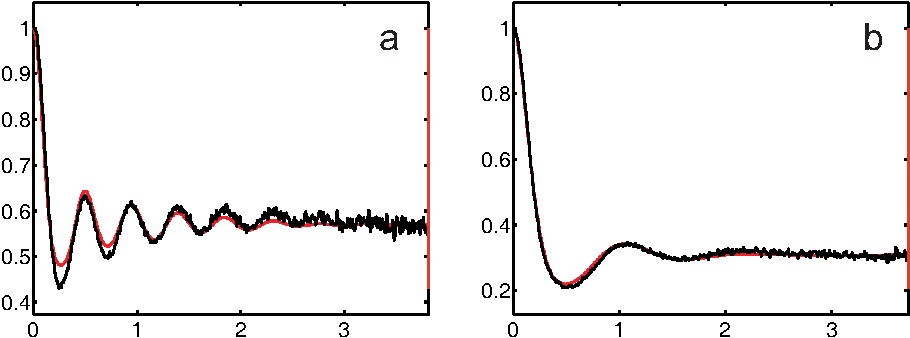
\includegraphics[width=0.62\textwidth]{figure12.pdf}
	\end{center}
	\caption{Spin counting via modulation depths. The modulation depth for data set {\ttfamily biradical} (a) is smaller than for data set {\ttfamily triradical} (b).}
	\label{fig:12}
\end{figure}

\subsection{Worked example: Calibration of spin counting}

\begin{itemize}
	\item Load data set {\ttfamily biradical} and optimize the range for background fitting. Optimize cutoff time (repeated clicking of the brown {\ttfamily !} button in the {\ttfamily \bf Original data} panel) and perform a Tikhonov regularization with L curve computation. Select a regularization parameter of 0.1. The normalized background-corrected signal decays to approximately 0.57 (Figure \ref{fig:12}a), corresponding to a modulation depth $\lambda \approx 0.43$.
	\item The {\ttfamily Number of spins} edit field now displays the number 2.05 in red color. This is very close to the expected number of 2 for a biradical, as this measurement was done under the standard conditions of the lab in which the program DeerAnalysis was developed. For a measurement at a different spectrometer, the number would deviate more strongly. 
	\item Write {\ttfamily 2.0} into the {\ttfamily Number of spins} edit field and press return. The updated number is displayed in green. Spin counting is now calibrated.
	\item Load data set {\ttfamily triradical}. Adjust zero time to 128 ns and optimize the background range. Optimize cutoff. With the modulation depth determined by APT, the spin count is 3.12. 
	\item Perform a Tikhonov regularization with L curve computation. Select a regularization parameter of 100. Here, the normalized background-corrected signal decays to approximately 0.3 (Figure \ref{fig:12}b), corresponding to a modulation depth $\lambda \approx 0.7$. The spin count changes only slightly to 3.13. Generally, the error in spin counting due to variations in the experimental conditions, e.g., different width of the resonator mode due to different overcoupling is larger than the difference between the APT result and optimized Tikhonov regularization. 
\end{itemize}

\subsection{Problem: Determining the number of spins in unknown samples}

\subsubsection*{Problem}
Using the calibration made above and APT, determine the number of spins for data sets (a) {\ttfamily sampleX} and (b) {\ttfamily deer\_broad\_50K\_4us}. Interpret the result for the latter data set, which stems from a sample of spin-labelled gold nanoparticles.

\subsubsection*{Answer}
(a) 2.05. The sample is a biradical.
(b) 1.39. There are two aspects with respect to interpretation. First, if correct, the number would correspond to the \emph{average} number of spin labels per nanoparticle. Second, part of the contribution at short distances will be lost. The computed number is thus expected to be lower than the actual average number of spin labels per nanoparticle. Indeed, when using Tikhonov regularization with excitation bandwidth correction and $\alpha=10000$, one finds a slightly larger number of 1.42. Generally, different values for the number of spins with and without excitation bandwidth correction point to the fact that contributions from short distances are underestimated. This correction cannot, however, recover the value of the modulation depth corresponding to ideal pulses.

\section{Using single label data}
There are two reasons why one may want to perform a DEER experiment on a singly labelled sample, which has only a background decay but no defined dipolar evolution. First, the background decay contains information on the concentration of spin labels. Second, for a protein the actual background function may differ from the function expected for a homogeneous distribution of point-like particles in space. By measuring data for the single mutants, one can obtain an experimental background function that can later be used for correcting the data for double mutants.

\subsection{Worked example: Determining concentrations}
Similar to modulation depths, the rate of background decay depends on pulse lengths, correct flip angle of the pump pulse, and shape of the nitroxide spectrum. Concentration measurements thus need to be calibrated.

\begin{figure}[ht]
 \vspace{10mm}
 	\begin{center}
		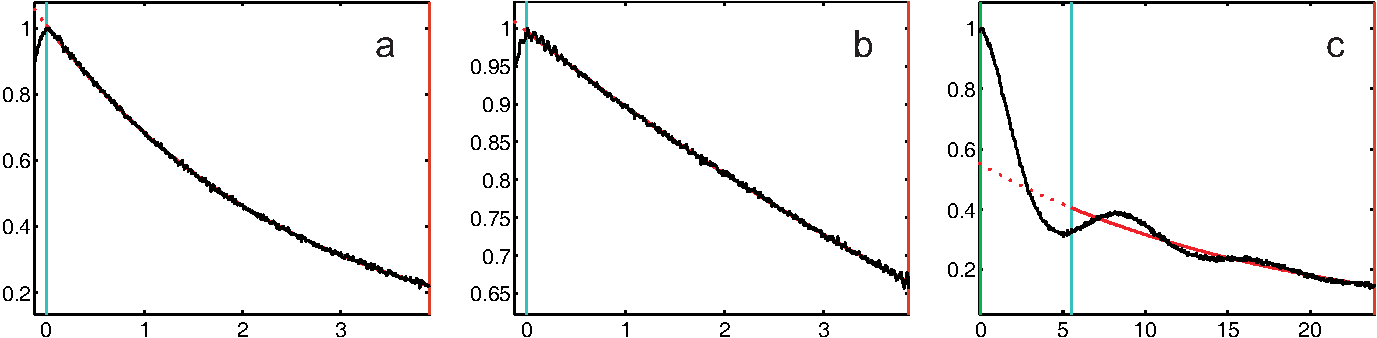
\includegraphics[width=0.95\textwidth]{figure13.pdf}
	\end{center}
	\caption{Determination of concentrations by exponential background fitting.  (a) Calibration data set {\ttfamily tempol\_toluene\_2500uM} (b) Data set {\ttfamily monoradical} with a concentration of about 670 $\mu$mol L$^{-1}$. (c) Data set {\ttfamily deer\_long\_50K} with a concentration of about 350 $\mu$mol L$^{-1}$}
	\label{fig:13}
\end{figure}

\begin{itemize}
	\item Load data set {\ttfamily tempol\_toluene\_2500uM}. This sample was prepared by dissolving 2 mmol L$^{-1}$ TEMPOL in toluene and shock-freezing the solution. As the toluene glass at 80 K has only about 80\% of the volume of the solution at room temperature, the actual concentration is 2.5 mmol L$^{-1}$. 
	\item  Correct the zero time to 128 ns and then set the start for background fitting to 0 ns by direct input into the blue edit field in the {\ttfamily \bf Original data} panel (Figure \ref{fig:13}a). The {\ttfamily Density} edit field in the {\ttfamily \bf Background model} panel now shows a value of 2.516. Correct this value to 2.5 by direct input into the edit field and press Return. The updated number is now shown in green colour. Concentration measurements are now calibrated for the experimental parameters used in the measurement of sample {\ttfamily tempol\_toluene\_2500uM}.
	\item Load data set {\ttfamily deer\_long\_50K}. Correct the zero time to 96 ns and then optimize the range for background fitting (blue {\ttfamily !} button in the {\ttfamily \bf Original data} panel, Figure \ref{fig:13}c). For this sample, the concentration is about 350 $\mu$mol L$^{-1}$.  
\end{itemize}

\subsection{Worked example: Deriving and using an experimental background function}


\begin{figure}[ht]
 \vspace{10mm}
 	\begin{center}
		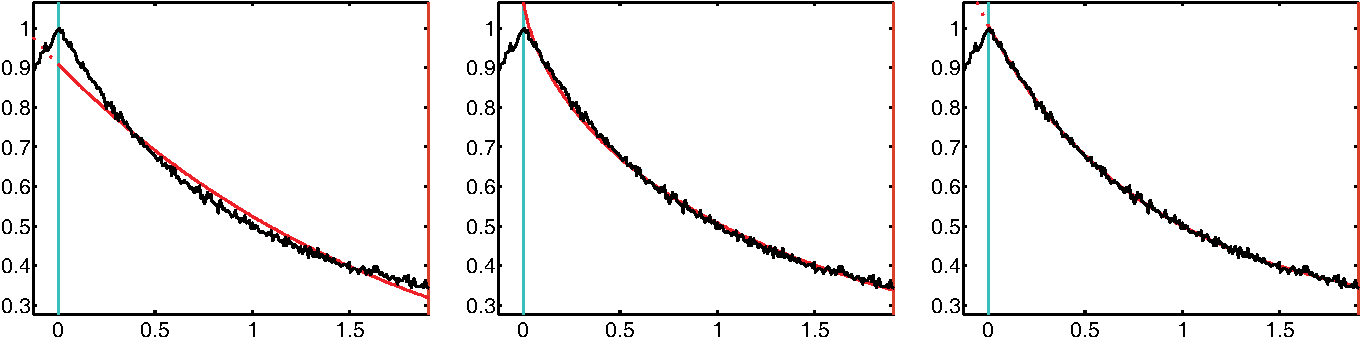
\includegraphics[width=0.95\textwidth]{figure14.pdf}
	\end{center}
	\caption{Different background models fitted to data set {\ttfamily monolabel\_41} obtained on a membrane protein singly-labelled at position 41.  (a) Fit by an exponential decay corresponding to a homogeneous distribution of point-like labels in space. (b) Fit by a stretched exponential decay corresponding to a homogeneous distribution of point-like labels in a plane. (c) Fit of the logarithm of the data by a 5$^{th}$ order polynomial.}
	\label{fig:14}
\end{figure}

\begin{itemize}
	\item Load data set {\ttfamily monolabel\_41}. This data set was obtained on a membrane protein singly labelled at residue 41. Set zero time to 128 ns and start of the background fit to 0 ns. The decay cannot be fit by a homogeneous distribution in three dimensions (Figure \ref{fig:14}a).
	\item Change the value in the edit field {\ttfamily Homogeneous dimensions} of the {\ttfamily \bf Background model} panel to 2. The fit improves significantly (Figure \ref{fig:14}a). This is because the distribution of a membrane protein in a liposome on the length scale of DEER is much closer to a homogeneous distribution in two dimensions than to a homogeneous distribution in three dimensions \cite{hilger2005}. Yet, a close look reveals that even the two-dimensional homogeneous distribution does not perfectly fit the decay (Figure \ref{fig:14}b).
	\item Select the {\ttfamily Fit dimens. checkbox} in the {\ttfamily Homogeneous dimensions} subpanel of the {\ttfamily \bf Background model} panel. The dimension changes to 2.14. The fit further improves, but is still not perfect. The improvement is because unilamellar vesicles are not perfectly flat and because the spin labels feature some spatial distribution along the bilayer normal. Hence, the effective dimension of the distribution is slightly larger than 2.0 (and may vary with labeling position). The still imperfect fit is due to excluded volume effects. A homogeneous distribution assumes that spin labels can approach each other very closely. However, the bulk of the protein prevents that, hence short distances are underrepresented.	
	\item Select the {\ttfamily Polynomial} radiobutton in the {\ttfamily \bf Background model} panel. The logarithm of the original data is now fitted by a 5$^\mathrm{th}$ order polynomial. This provides an almost perfect fit (Figure \ref{fig:14}c). To see the fit residual in the {\ttfamily \bf Form factor} plot better, select {\ttfamily Tikhonov reg.} in the {\ttfamily \bf Distance analysis} panel. Except for noise, the residual is flat.
	\item Decrease {\ttfamily Polynomial order}, watching the {\ttfamily r.m.s. value} in the {\ttfamily \bf Background model} panel. A polynomial order as low as 3 provides a fit with the same quality, for a polynomial order of 2 the rm.s. value increases and the initial part of the fit residual (first 0.4 $\mu$s) is no longer flat. Hence, set polynomial order to 3.  
	\item Click on the {\ttfamily Save} button in to the {\ttfamily Polynomial} subpanel and save the background polynomial as {\ttfamily bckg\_41}.  
	\item Load data set {\ttfamily monolabel\_423} and repeat the procedure. In this case, the optimum order of the polynomial is 5. Save this background polynomial as {\ttfamily bckg\_423}.
	\item Load data set {\ttfamily mix\_monolabel\_41\_423}. This data set was obtained on a mixture of the two singly labelled mutants. Set start of the background range to 0 ns and select the {\ttfamily Experimental} radiobutton in the {\ttfamily \bf Background model} panel. Using the {\ttfamily Load} button in the {\ttfamily Experimental subpanel}, load the background polynomial {\ttfamily bckg\_41}. The r.m.s. value for the fit with this background polynomial is 0.006379. At the beginning and at the end of the data, there are some deviations from a flat residual.   
	\item Load the background polynomial {\ttfamily bckg\_423}. The r.m.s. value for the fit with this background polynomial is 0.006687. The residual exhibits a slight oscillation.   
	\item Using the {\ttfamily Add} button in the {\ttfamily Experimental subpanel}, add the background polynomial {\ttfamily bckg\_41}. In the dialog window that pops up, input a weighting of 1.0 for this second background polynomial.\footnote{If labeling efficiency were different at these two positions and you would know that, you could adapt the weighting.} The r.m.s. value for the fit with the sum of the two single-label background polynomials improves to 0.006219. The sum of the two single-label polynomials would be almost perfect for fitting the background in a sample of the protein doubly labelled at positions 41 und 423. This background function could now be used for correction of the double mutant 41/423 (data set not contained in DeerAnalysis distribution).
\end{itemize}

\section{Worked example: Validation}

This is an example with a long computation time.

\begin{figure}[ht]
 \vspace{10mm}
 	\begin{center}
		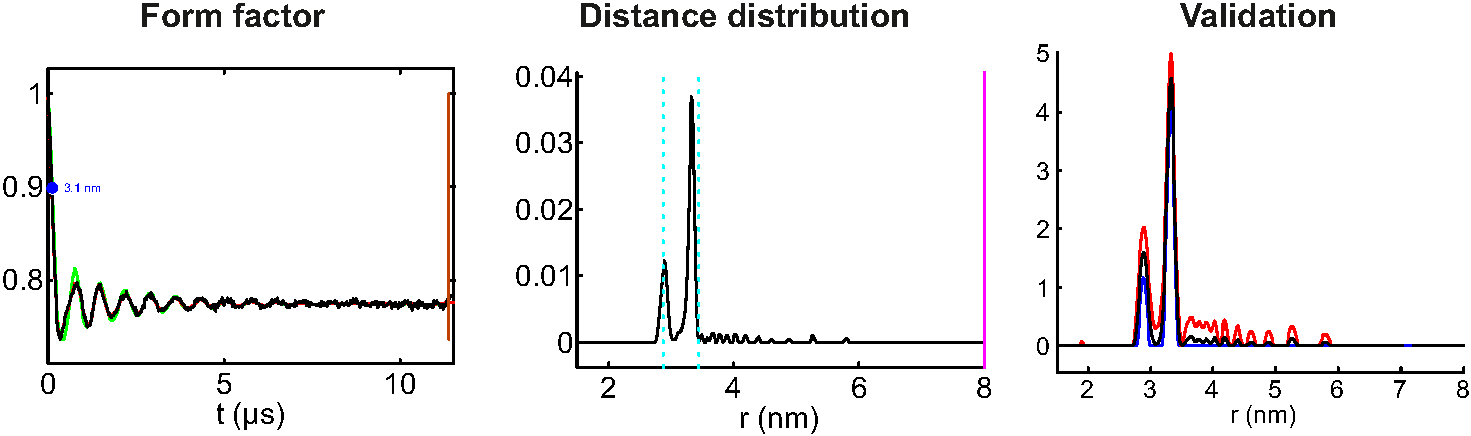
\includegraphics[width=0.95\textwidth]{figure15.pdf}
	\end{center}
	\caption{Validation of an (impurity) peak for data set {\ttfamily birad\_rigid\_DEER\_vs\_B0\_prj} obtained on a biradical during an early stage of syntehsis development.  (a) Experimental form factor (black), best fit corresponding to the complete distance distribution (red), and simulation with the peak between 2.7 and 3.1 nm suppressed (green). (b) Distance distribution. (c) Fit of the logarithm of the data by a 5$^{th}$ order polynomial.}
	\label{fig:15}
\end{figure}

\begin{itemize}
	\item Load data set {\ttfamily birad\_rigid\_DEER\_vs\_B0\_prj}. This data set was obtained on a biradical with conformationally unambiguous spin label \cite{jeschke2010} at an early stage of optimizing purification of the compound. The data were acquired with magnetic field averaging to diminish orientation selection effects. Therefeore the decay cannot be fit very well by a homogeneous distribution in three dimensions (Figure \ref{fig:15}a). Activate the {\ttfamily Fit dim.} checkbox in the {\ttfamily \bf Background model panel} and optimize the background range (this takes \emph{very} long.
	\item Perform Tikhonov regularization with L curve computation. The L curve does not look very well defined. Switch through the regularization parameters and observe the agreement between experimental and simulated {\ttfamily Form factor}. You will see that a regularization parameter of 0.1 or, perhaps, even 0.01 is appropriate. We use $\alpha = 0.1$ here.
	\item The distance distribution (Figure \ref{fig:15}b) exhibits two peaks at 2.86 and 3.30 nm a few minor peaks at larger distances.	A suppression test for the range from 2.7 to 3.1 nm (Figure \ref{fig:15}a,b) indicates that the peak at 2.86 nm is significant.
	\item Reset the {\ttfamily \bf Distance distribution} cursosr to 1.5 to 8 nm by clicking the respective {\ttfamily !} buttons. Now click the {\ttfamily Validation} button in the {\ttfamily \bf Distance analysis} panel. A new window {\ttfamily Tikhonov validation with regularization parameter 0.1} opens. Deactivate the {\ttfamily Background density} and {\ttfamily Modulation depth} checkboxes and activate the {\ttfamily White noise} checkbox. Edit the {\ttfamily Trial number} for {\ttfamily White noise} to 10. The number {\ttfamily Total trials} should update to 10. You will thus perform a validation for noise effects only, assuming that the background correction is not responsible for the questionable peaks. This is a good assumption in the case at hand. Click the {\ttfamily Compute} button to perform the validation. This will take a while.
	\item After the computation has finished, the {\ttfamily \bf Distance distribution} plot in the validation window now shows the mean distance distribution (black), a lower estimate (blue) and an upper estimate(red) (Figure \ref{fig:15}c), which were obtained by ten trials with doubled noise level.\footnote{This is better seen when you detach the plot with the {\ttfamily Copy} button.} The noise level is increased by adding pseudorandom numbers to the experimental primary data. The lower estimate shows that the peak at 2.86 nm is very likely significant, while the small peaks at distances larger than 3.5 nm are most likely insignificant. Indeed the peak at 2.86 nm was reproducible in further measurements of the same sample, while the peaks at larger distances varied. By purification of the compound, the peak at 2.86 nm could be removed. It is due to a biradical with a shorter spacer.
	\item After you have closed the validation window with the {\ttfamily Close} button, the validation data are available in the main window (to prevent this from happening and preserve the original state of the main window, you would have to clsoe the window with the {\ttfamily Cancel} button). By activating the {\ttfamily error est.} checkbox in the {\ttfamily \bf Distance distribution} panel,you can visualize uncertainty of the distance distribution as grey error bars. Note that all analysis measures (e.g. mean distance and distribution width) now correspond to the mean distance distribution for all validation trials.  	 
\end{itemize}

Here the tutorial ends. Further features of DeerAnalysis2010 and some of the background theory are explained in the user manual. 

\section*{Acknowledgments}
All shape-persistent biradicals for the example data sets were prepared by A. Godt, University of Bielefeld \cite{godt2000}. The surface-labelled gold nanoparticles were prepared by P. Ionita and V. Chechik, University of York. The samples of plant light harvesting complex IIb were provided by A. Bender and H. Paulsen, University of Mainz. The samples and data sets for the singly-labelled membrane proteins were provided by D. Hilger and H. Jung, LMU Munich.

\begin{thebibliography}{00}

% \bibitem{label}
% Text of bibliographic item

% notes:
% \bibitem{label} \note

% subbibitems:
% \begin{subbibitems}{label}
% \bibitem{label1}
% \bibitem{label2}
% If there is a note, it should come last:
% \bibitem{label3} \note
% \end{subbibitems}

\bibitem{milov1981}
A.D. Milov, K.M. Salikhov, M.D. Shirov, 
{\em Fiz. Tverd. Tela (Leningrad)} {\bf 23} (1981) 957--982.

\bibitem{milovrev}
A. D. Milov, A. G. Maryasov, Yu. D. Tsvetkov, 
{\em Appl. Magn. Reson.} {\bf 15} (1998) 107--143.

\bibitem{pannier2000}
M. Pannier, S. Veit, A. Godt, G. Jeschke, H. W. Spiess,
{\em J. Magn. Reson.} {\bf 142} (2000) 331--340.

\bibitem{jeschke2002}
G. Jeschke,
{\em ChemPhysChem} {\bf 3} (2002) 927--932.

\bibitem{jeschkerev}
G. Jeschke,
{\em Macromol. Rapid Commun.} {\bf 23} (2002) 227--246.

\bibitem{jeschke2001}
G. Jeschke, A. Koch, U. Jonas, A. Godt,
{\em J. Magn. Reson.} {\bf 155} (2001) 72--82.

\bibitem{jeschke2004}
G. Jeschke, G. Panek, A. Godt, A. Bender, H. Paulsen,
{\em Appl. Magn. Reson.} {\bf 26} (2004) 223--244.

\bibitem{chiang2005}
Y. W. Chiang, P. P. Borbat, J. H. Freed,
{\em J. Magn. Reson.} {\bf 172} (2005) 279--295.

\bibitem{jeschke2006}
G. Jeschke, V. Chechik, P. Ionita, A. Godt, H. Zimmermann, J. Banham, C. R. Timmel, D. Hilger, H. Jung,
{\em Appl. Magn. Reson.} {\bf 30} (2006) 473--498.

\bibitem{jeschke2007}
G. Jeschke, Ye. Polyhach
{\em Phys. Chem. Chem. Phys.} {\bf 9} (2007) 1895--1910.

\bibitem{godt2006}
A. Godt, M. Schulte, H. Zimmermann, G. Jeschke,
{\em Angew. Chem. Int. Ed.} {\bf 45} (2006) 7560-7564.

\bibitem{godt2000}
A. Godt, C. Franzen, S. Veit, V. Enkelmann, M. Pannier, G. Jeschke,
{\em J. Org. Chem.} {\bf 65} (2000) 7575--7582.

\bibitem{milov1984}
A. D. Milov, A. B. Ponomarev, Yu. D. Tsvetkov,
{\em Chem. Phys. Lett.} {\bf 110} (1984) 67--72.

\bibitem{hilger2005}
D. Hilger, H. Jung, E. Padan, C. Wegener, K.-P. Vogel, H.-J. Steinhoff, G. Jeschke, 
{\em Biophys. J.} {\bf 89} (2005) 1328--1338.

\bibitem{bode2007}
B. E. Bode, D. Margraf, J. Plackmeyer, G. Durner, T. F. Prisner, O. Schiemann, 
{\em J. A. Chem. Soc.} {\bf 129} (2007) 6736--6745.

\bibitem{jeschke2010}
G. Jeschke, M. Sajid, M. Schulte, N. Ramezanian, A. Volkov, H. Zimmermann,  A. Godt, 
{\em J. A. Chem. Soc.} {\bf 132} (2010) 10107--10117.

\end{thebibliography}

\end{document}